\section{Auswertung}
\label{sec:Auswertung}
\subsection{Ermittelung der mittleren freien Weglänge}
Die mittlere freie Weglänge der Elektronen kann mithilfe von 
Formel (\ref{eqn:Sättigungsdampfdruck}) und (\ref{eqn:mittlereWeglängeAtome}) 
berechnet werden. Die dazu verwendeten 
Temperaturen $T$, bei denen die Kurven aufgenommen werden, 
sind in Tabelle (\ref{tab:Weglaenge}) zusammen mit den Ergbenissen 
aufgelistet. Außerdem wird das Verhältnis aus dem Abstand 
$a = 1 \, \unit{\centi\meter}$ zwischen Kathode und 
Elektrode und der mittleren freien Weglänge berechnet 
und in Tabelle (\ref{tab:Weglaenge}) aufgelistet.           
\begin{table}[H]
    \centering
    \caption{Mittlere freie Weglänge mit Verhältnis.}
    \label{tab:Weglaenge}
    \begin{tblr}{colspec={c c c}}
        \toprule
        $\text{T} \left[\unit{\kelvin}\right]$ & $\bar{\omega} \left[\unit{\meter}\right]$ & $a/ \bar{\omega}$\\
        \midrule  
        $295,75$ & $6,59 \cdot 10^{-3}$ & $1,52$\\ 
        $423,15$ & $6,01 \cdot 10^{-6}$ & $1,66 \cdot 10^{3}$\\ 
        $433,15$ & $4,13 \cdot 10^{-6}$ & $2,42 \cdot 10^{3}$\\ 
        $444,15$ & $2,79 \cdot 10^{-6}$ & $3,59 \cdot 10^{3}$\\ 
        $451,15$ & $2,19 \cdot 10^{-6}$ & $4,56 \cdot 10^{3}$\\ 
        $453,15$ & $2,05 \cdot 10^{-6}$ & $4,88 \cdot 10^{3}$\\
        \bottomrule
    \end{tblr}
\end{table}
Das Verhältnis nimmt mit steigender Temperatur zu. 
\subsection{Differentielle Energieverteilung}
Die zugrundeliegende Messkurve wird mithilfe eines 
x-y-Schreibers aufgezeichnet. Die Messkurve, die bei einer 
Temperatur von $22,6 \, °\text{C}$ aufgenommen wird, ist 
in Abbildung (\ref{fig:22,6}) zu sehen. Die Messkurve, die bei 
$150 \, °\text{C}$ aufgenommen wird, ist in Abbildung 
(\ref{fig:150}) zu sehen. Beide Kurven werden bei einer
Beschleunigungsspannung von $U_B = 11 \, \unit{\volt}$
aufgenommen. Da die Daten nur graphisch vorliegen, 
müssen sie vom Papier abgelesen werden. 
\begin{figure}[H]
    \centering
    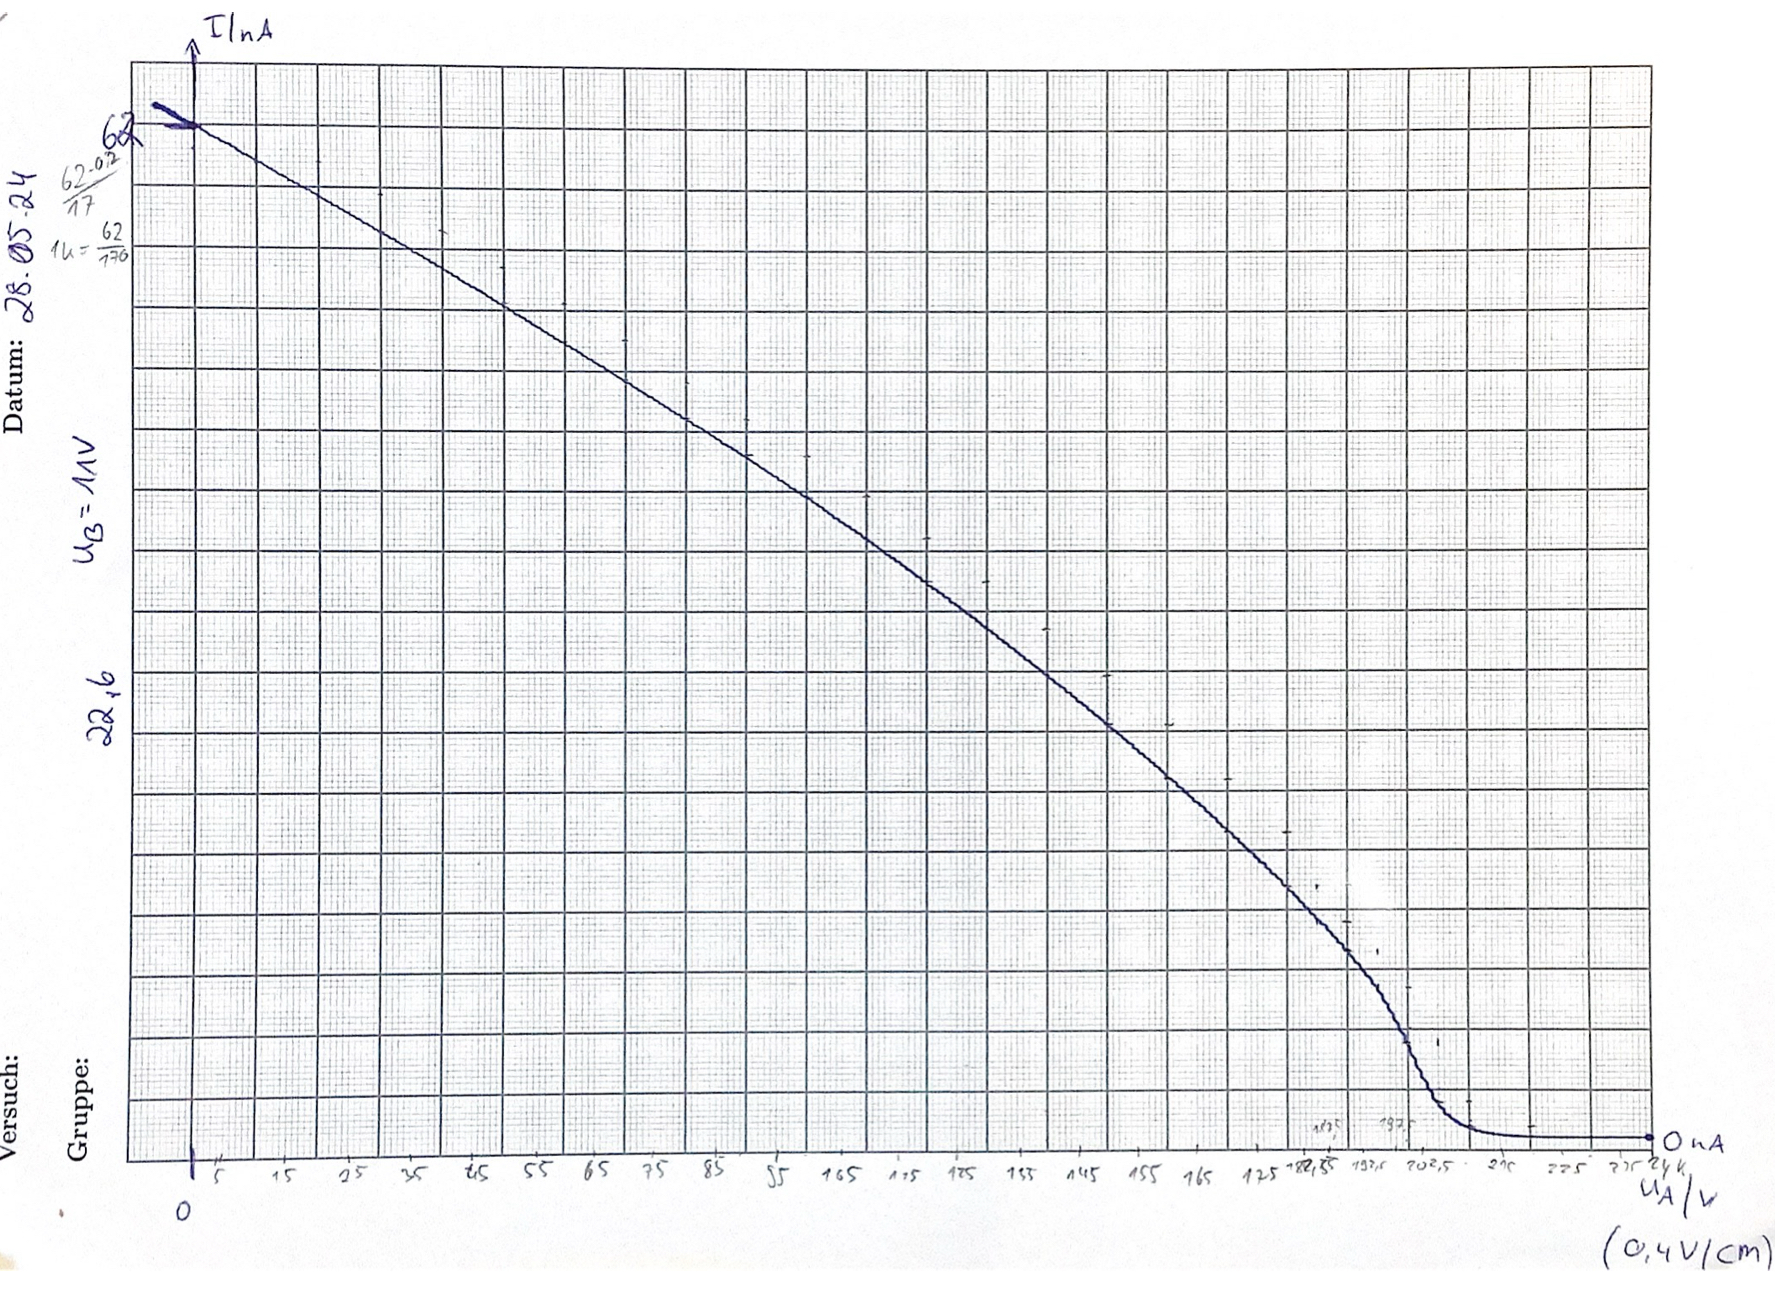
\includegraphics[width=0.8\textwidth]{content/Bilder/22,6.jpeg}
    \caption{Strom-Spannungsmesskurve bei T = 22,6 °C.}
    \label{fig:22,6}
\end{figure}
\begin{figure}[H]
    \centering
    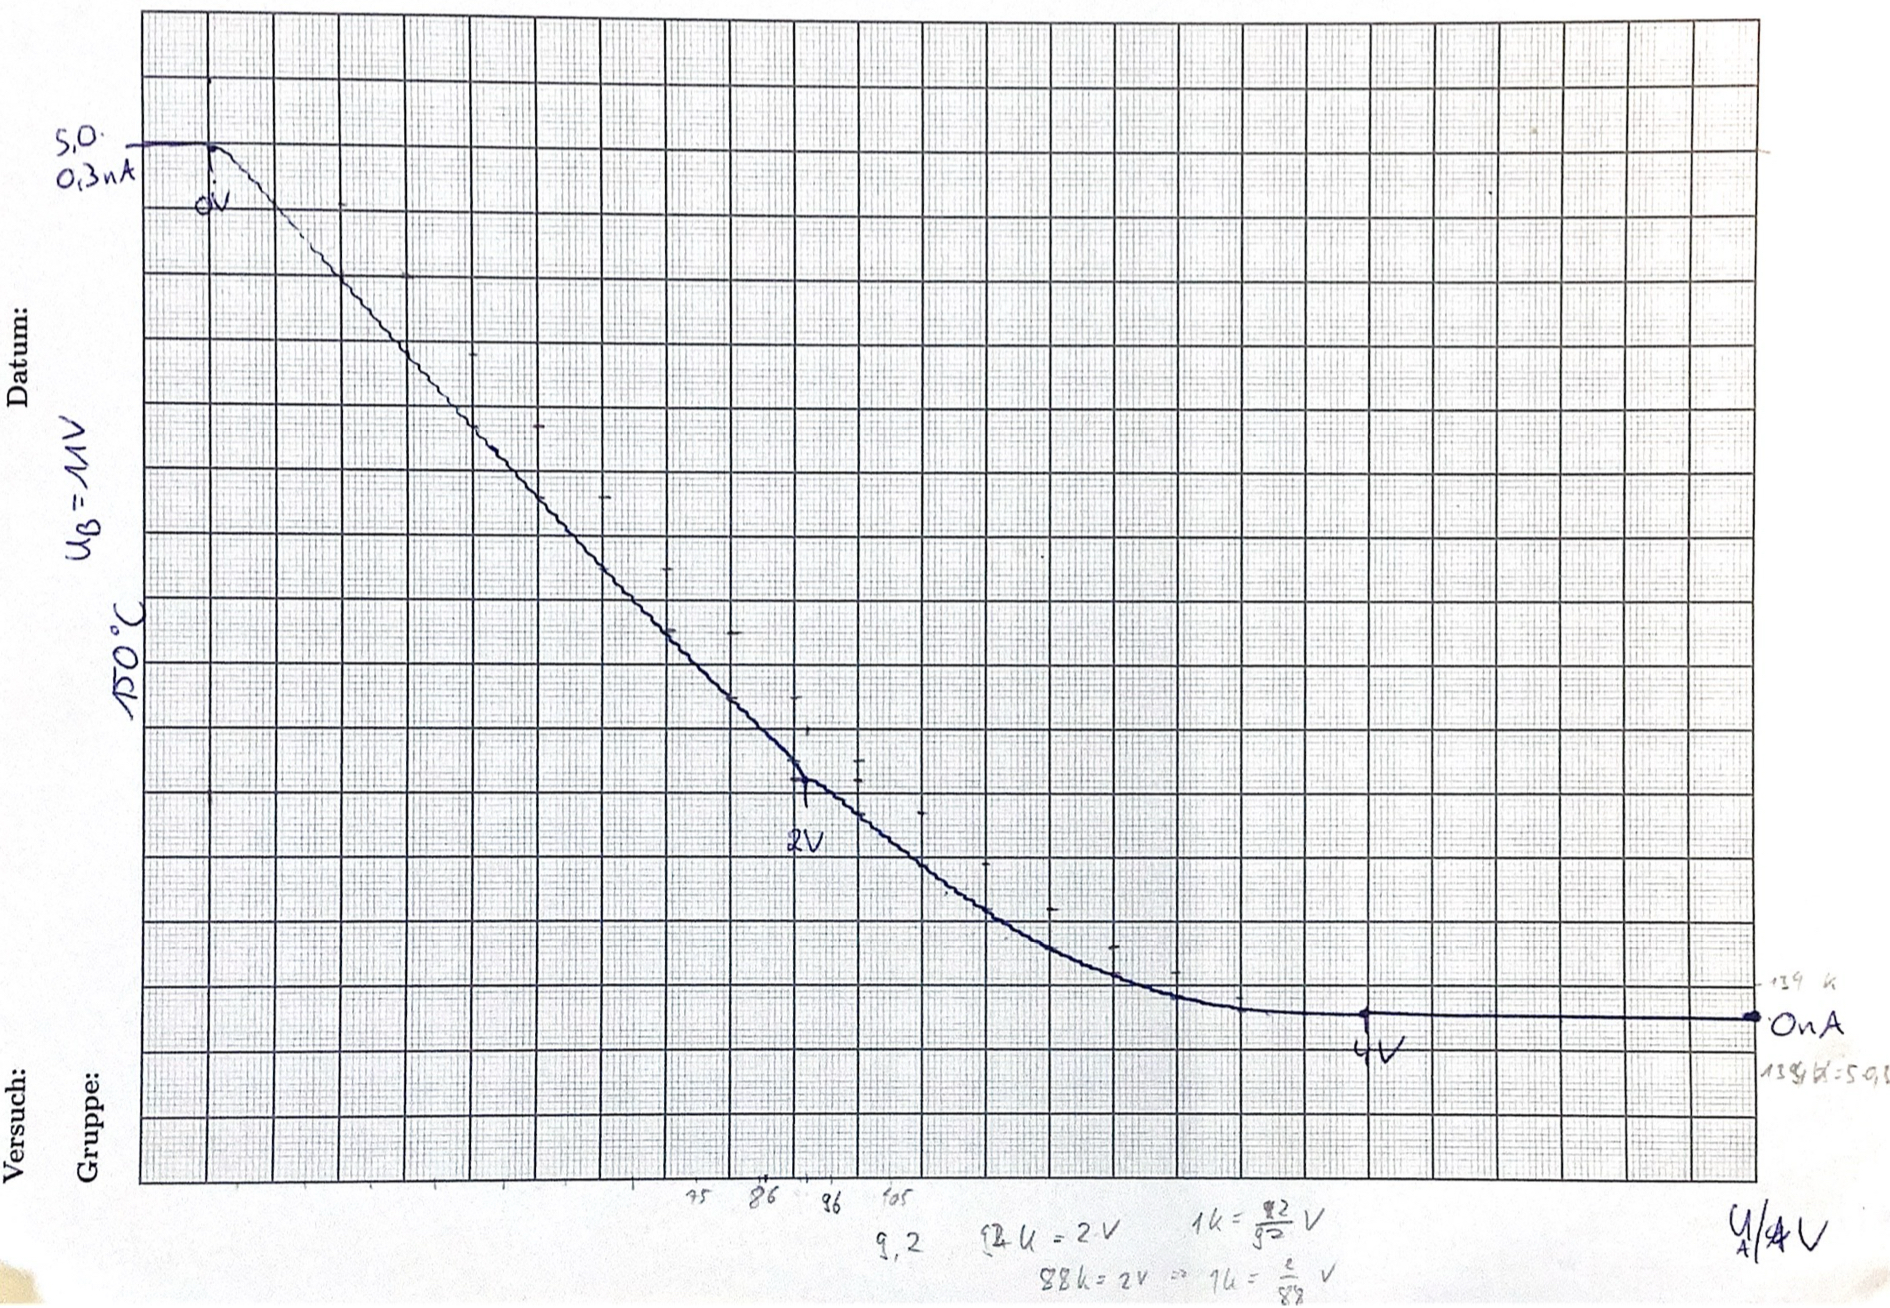
\includegraphics[width=0.8\textwidth]{content/Bilder/150.jpeg}
    \caption{Strom-Spannungsmesskurve bei T = 150 °C.}
    \label{fig:150}
\end{figure}
Die errechnete Steigung und der zugehörige Spannungswert 
sind für die Kurve bei $22,6 \, °\text{C}$ und für $150 \, °\text{C}$ in 
Tabelle (\ref{tab:22,6_Steigung}) vermerkt. Diese Werte für die Kurve von $22,6 \, °\text{C}$ sind 
in Abbildung (\ref{fig:22,6_Steigung}) dargestellt. 
\begin{table}[H]
    \centering
    \caption{Steigung der Kurve bei 22,6 °C und 150 °C in Abhängigkeit von der Spannung.}
    \label{tab:22,6_Steigung}
    \begin{tblr}{colspec={c c | c c}}
        \toprule
        $U_{22,6} \left[\unit{\volt}\right]$ & $I_{22,6}/U_{22,6} \left[\unit{\ampere\per\volt}\right]$ & $U_{150} \left[\unit{\volt}\right]$ & $I_{150}/U_{150} \left[\unit{\ampere\per\volt}\right]$\\
        \midrule  
        0,2 & 5,45 & 0,11 & 0,46  \\
        0,6 & 4,54 & 0,33 & 0,57  \\
        1   & 5,45 & 0,54 & 0,62  \\
        1,4 & 5,45 & 0,76 & 0,57  \\
        1,8 & 5,45 & 0,98 & 0,57  \\
        2,2 & 5,45 & 1,20 & 0,57  \\
        2,6 & 6,36 & 1,41 & 0,51  \\
        3   & 5,45 & 1,63 & 0,51  \\
        3,4 & 5,45 & 1,87 & 0,56  \\
        3,8 & 6,36 & 2,18 & 0,31  \\
        4,2 & 6,36 & 2,39 & 0,39  \\
        4,6 & 6,36 & 2,61 & 0,34 \\
        5   & 7,27 & 2,84 & 0,30  \\
        5,4 & 6,36 & 3,07 & 0,20  \\
        5,8 & 7,27 & 3,30 & 0,20  \\
        6,2 & 8,18 & 3,52 & 0,10  \\
        6,6 & 8,18  & 3,75 & 0 \\
        7   & 8,18  & 3,98 & 0 \\
        7,3 & 10,91 & 4,20 & 0  \\
        7,5 & 9,09  & 4,43 & 0 \\
        7,7 & 10,91 & 4,66 & 0  \\
        7,9 & 16,36 & 4,89 & 0  \\
        8,1 & 18,18 & 5,11 & 0  \\
        8,3 & 7,27  & 5,34 & 0 \\
        8,6 & 1,82 & & \\
        9  & 0 & & \\
        9,4 & 0 & & \\
        \bottomrule
    \end{tblr}
\end{table}
\begin{figure}[H]
    \centering
    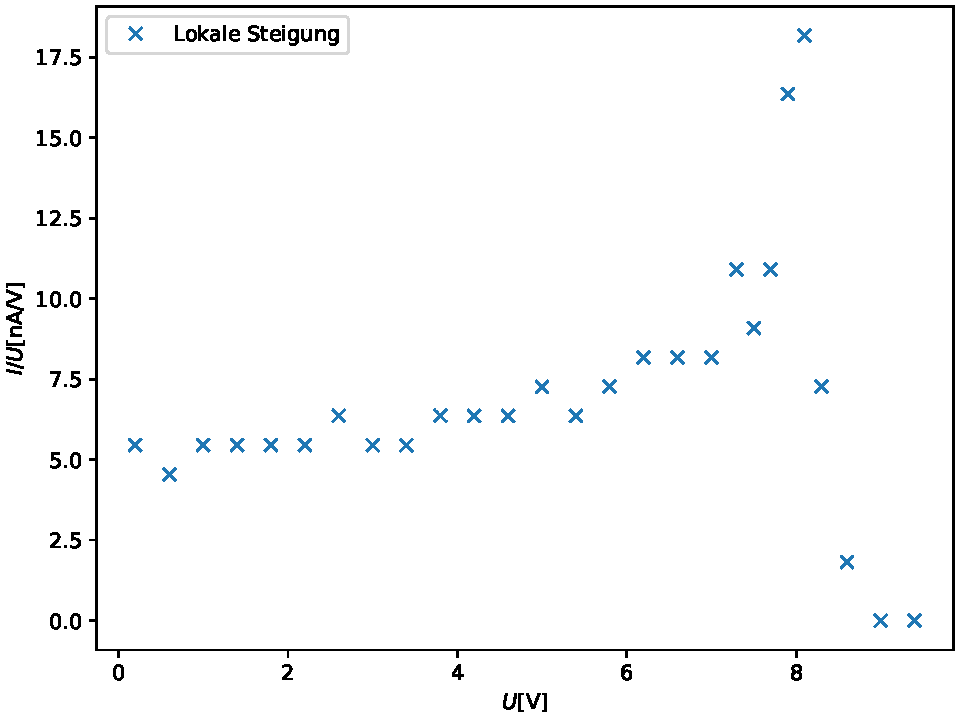
\includegraphics[width=0.8\textwidth]{plot1.pdf}
    \caption{Steigung der Kurve in Abhängigkeit von der Spannung bei 22,6 °C.}
    \label{fig:22,6_Steigung}
\end{figure}

Die Werte der Kurve bei $150 \, \unit{\celsius}$ sind 
in Abbildung (\ref{fig:150_Steigung}) dargestellt. 

\begin{figure}[H]
    \centering
    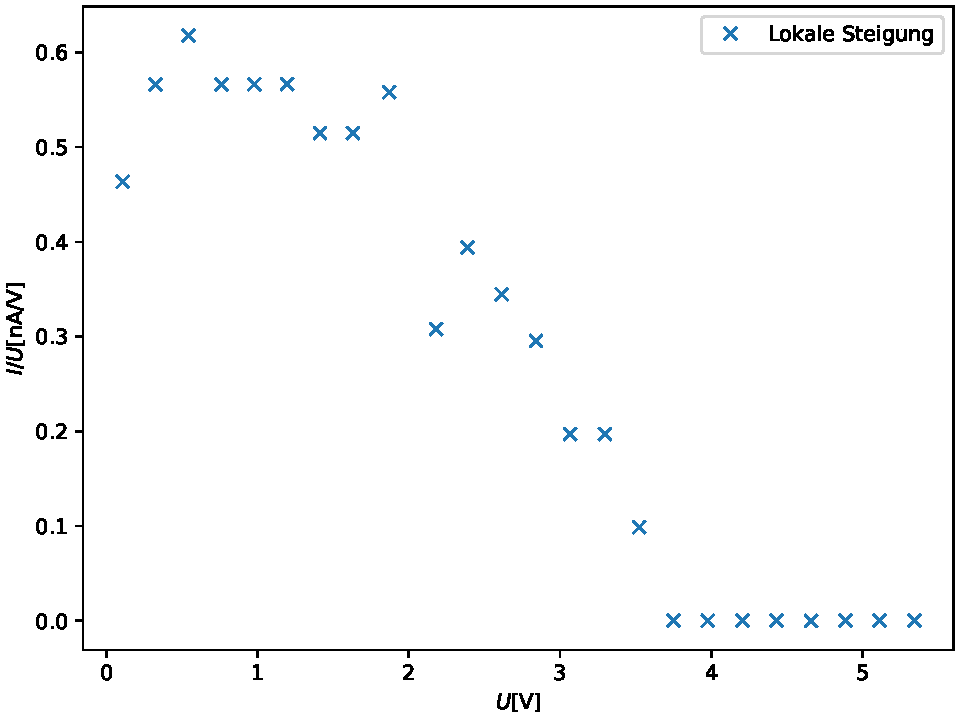
\includegraphics[width=0.8\textwidth]{plot2.pdf}
    \caption{Steigung der Kurve in Abhängigkeit von der Spannung bei 150 °C.}
    \label{fig:150_Steigung}
\end{figure}
Mithilfe des Spannungswertes der größten Steigung der Kurve bei $22,6 \, \unit{\celsius}$ wird das Kontaktpotential berechnet. 
Dazu wird Formel (\ref{eqn:Effektivspannung}) verwendet. Dies ergibt daher den Wert
$$U_K = 11 \, \unit{\volt} - 8,1  \, \unit{\volt} = 2,9 \, \unit{\volt}\, .$$
\subsection{Franck-Hertz-Kurve und Anregungsenergie}
Die Grundlage dieses Abschnitts der Auswertung sind 
Franck-Hertz-Kurven, die in Abbildung (\ref{fig:verschiedene}) zu 
sehen ist. 
\begin{figure}[H]
    \centering
    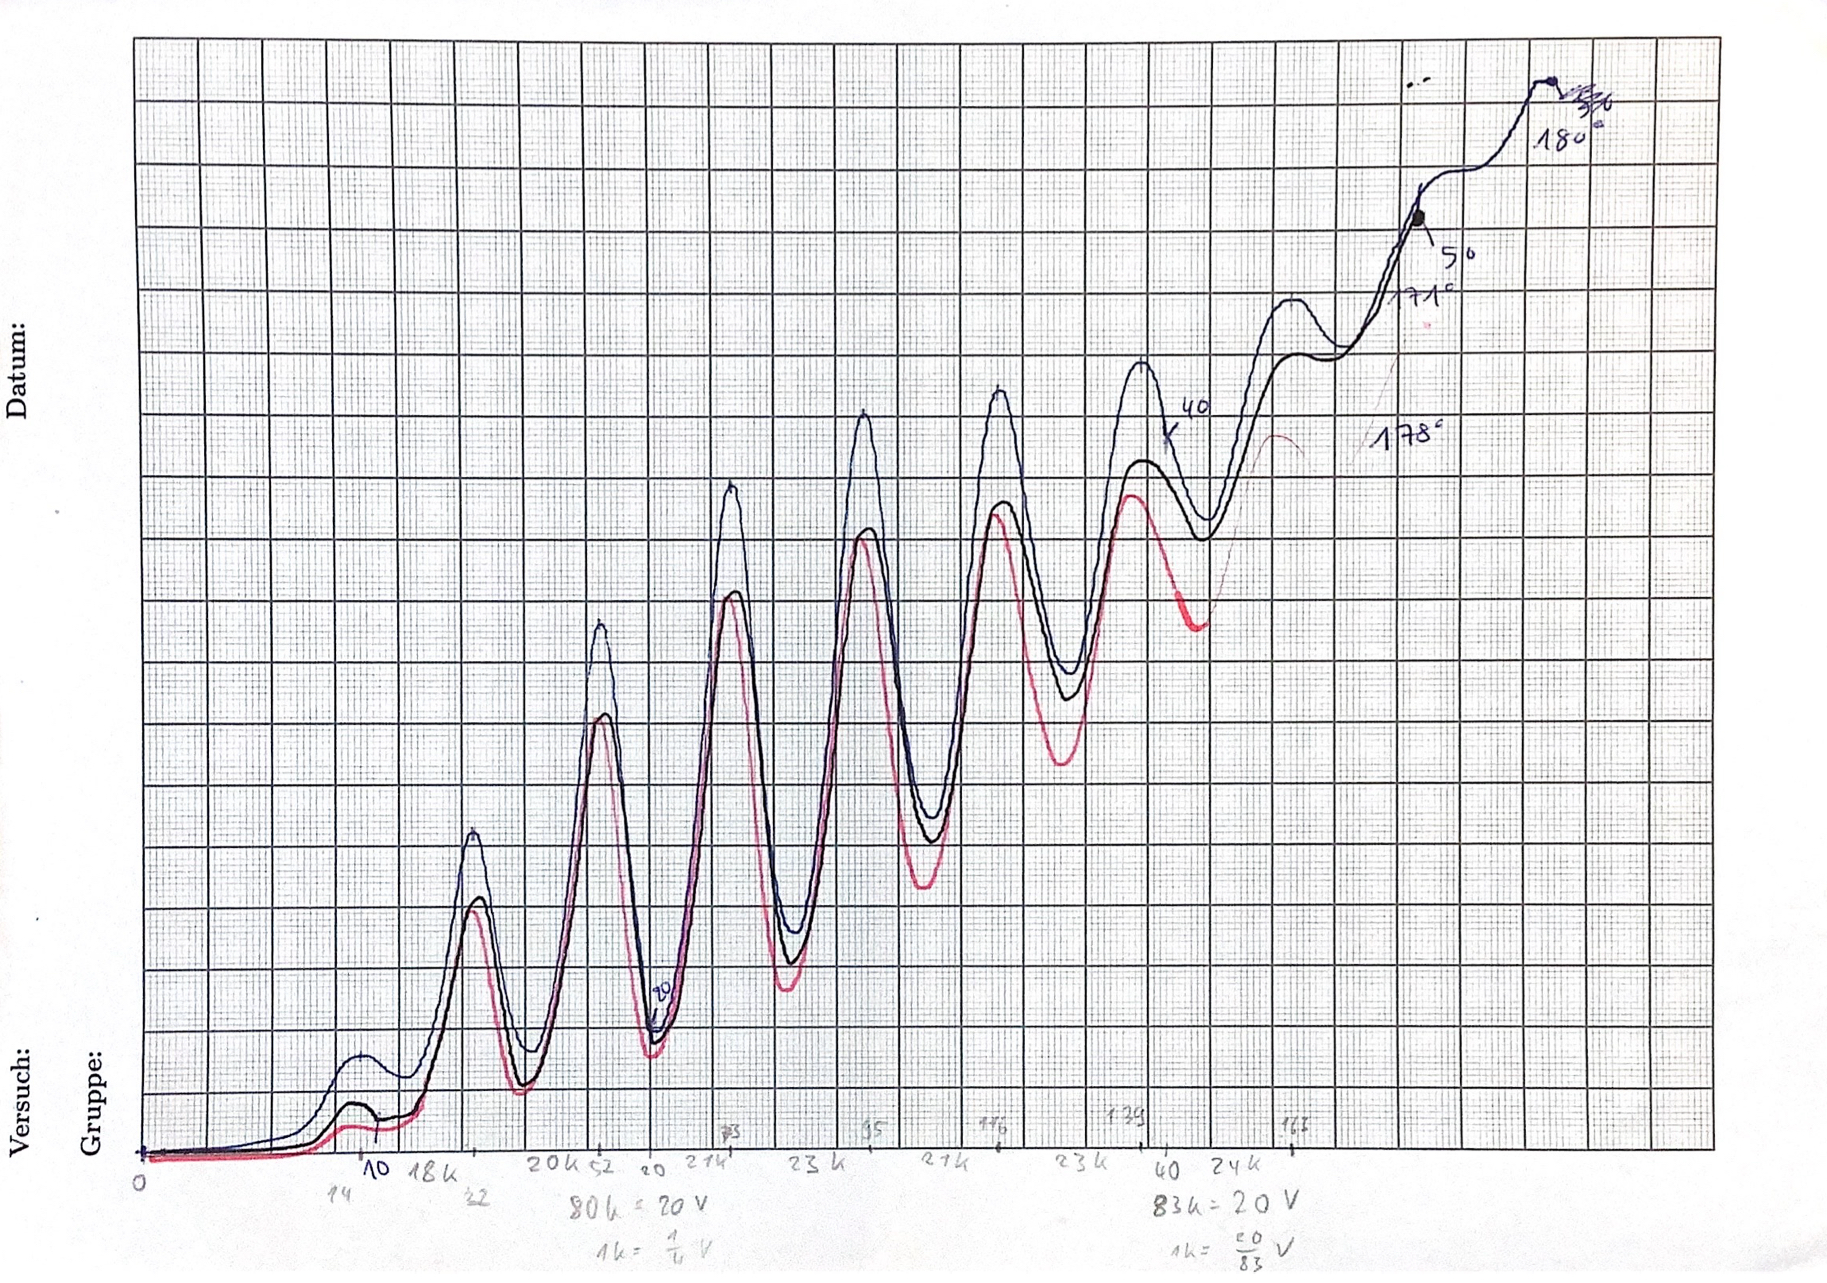
\includegraphics[width=0.8\textwidth]{content/Bilder/verschiedene.jpeg}
    \caption{Franck-Hertz-Kurven bei unterschiedlichen Temperaturen.}
    \label{fig:verschiedene}
\end{figure}
Zur Auswertung wird die obere, blaue Kurve ausgewählt, da die Maxima 
am deutlichsten sind. Die x-Position des N-ten Maximum ist in Tabelle (\ref{tab:franck}) dargestellt. 

\begin{table}[H]
    \centering
    \caption{x-Position des N-ten Maximum.}
    \label{tab:franck}
    \begin{tblr}{colspec={c c}}
        \toprule
        $\text{N-tes Maximum} $ & $\text{x-Position des Maximum} \left[\unit{\volt}\right]$ \\
        \midrule  
        1 & 3,5 \\
        2 & 8 \\
        3 & 13 \\
        4 & 17,59 \\
        5 & 22,89 \\
        6 & 27,95 \\
        7 & 33,49 \\
        8 & 39,27 \\
        \bottomrule
    \end{tblr}
\end{table}
Diese Werte sind in der Abbildung (\ref{fig:Maxima}) zu sehen mit Ausgleichsgerade der Form $y = mx + n$. 
Die Steigung der Ausgleichsgerade ist der mittlere Abstand der Maxima. 
\begin{figure}[H]
    \centering
    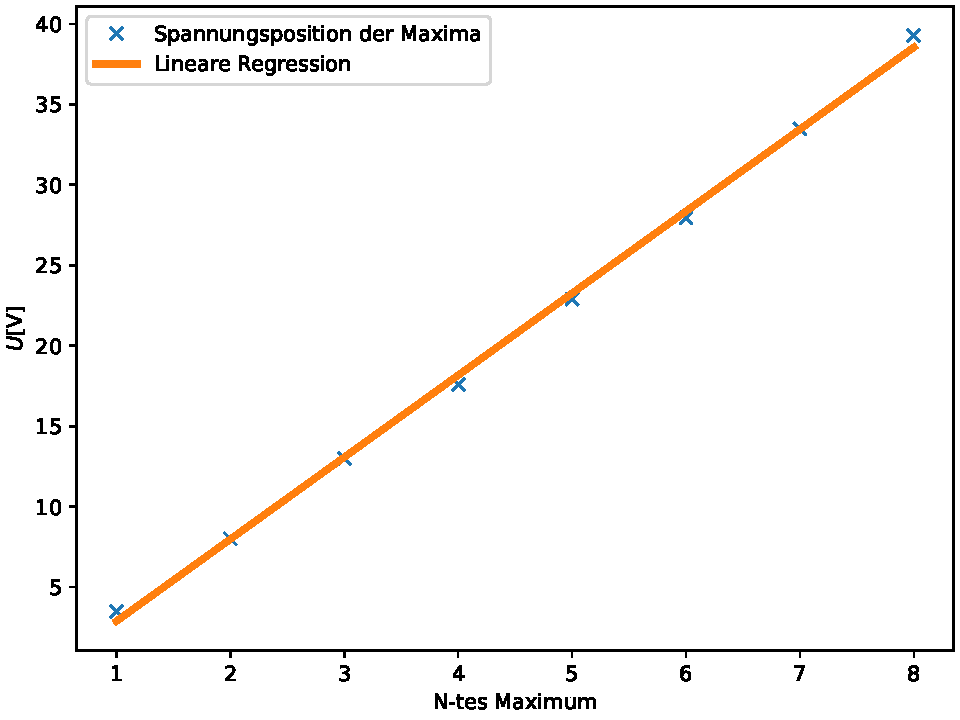
\includegraphics[width=0.8\textwidth]{plot3.pdf}
    \caption{Maxima einer Franck-Hertz-Kurve.}
    \label{fig:Maxima}
\end{figure}
Die berechneten Werte sind 
\begin{align*}
    m &= 5,1 \pm 0,08 \\
    n &= -2,2 \pm 0,4 \, .\\
\end{align*}
Daher gilt für die mittlere Beschleunigungsspannung
$(5,1 \pm 0,08) \unit{\volt}$. 
Aus dieser lässt sich die Wellenlänge durch 
$$\lambda = \frac{h \cdot c}{U_B \cdot e}$$ 
bestimmen. 
Es ergibt sich ein Wert von $\lambda = 2,43 \cdot 10^{-7} \unit{\meter}$. 
